% This is "sig-alternate.tex" V2.0 May 2012
% This file should be compiled with V2.5 of "sig-alternate.cls" May 2012
%
% This example file demonstrates the use of the 'sig-alternate.cls'
% V2.5 LaTeX2e document class file. It is for those submitting
% articles to ACM Conference Proceedings WHO DO NOT WISH TO
% STRICTLY ADHERE TO THE SIGS (PUBS-BOARD-ENDORSED) STYLE.
% The 'sig-alternate.cls' file will produce a similar-looking,
% albeit, 'tighter' paper resulting in, invariably, fewer pages.
%
% ----------------------------------------------------------------------------------------------------------------
% This .tex file (and associated .cls V2.5) produces:
%       1) The Permission Statement
%       2) The Conference (location) Info information
%       3) The Copyright Line with ACM data
%       4) NO page numbers
%
% as against the acm_proc_article-sp.cls file which
% DOES NOT produce 1) thru' 3) above.
%
% Using 'sig-alternate.cls' you have control, however, from within
% the source .tex file, over both the CopyrightYear
% (defaulted to 200X) and the ACM Copyright Data
% (defaulted to X-XXXXX-XX-X/XX/XX).
% e.g.
% \CopyrightYear{2007} will cause 2007 to appear in the copyright line.
% \crdata{0-12345-67-8/90/12} will cause 0-12345-67-8/90/12 to appear in the copyright line.
%
% ---------------------------------------------------------------------------------------------------------------
% This .tex source is an example which *does* use
% the .bib file (from which the .bbl file % is produced).
% REMEMBER HOWEVER: After having produced the .bbl file,
% and prior to final submission, you *NEED* to 'insert'
% your .bbl file into your source .tex file so as to provide
% ONE 'self-contained' source file.
%
% ================= IF YOU HAVE QUESTIONS =======================
% Questions regarding the SIGS styles, SIGS policies and
% procedures, Conferences etc. should be sent to
% Adrienne Griscti (griscti@acm.org)
%
% Technical questions _only_ to
% Gerald Murray (murray@hq.acm.org)
% ===============================================================
%
% For tracking purposes - this is V2.0 - May 2012

\documentclass{sig-alternate}

\usepackage{graphicx}
\usepackage{amsmath}
\usepackage[skip=5pt]{caption}
%\usepackage{hyperref}
\usepackage{enumitem}
\usepackage{url}



\newcommand{\todo}[1]{\textbf{[[#1]]}}
\newcommand{\pseudosection}[1]{\vspace{0.5\baselineskip} \noindent {\bf #1}}


\begin{document}
% --- Author Metadata here ---
\conferenceinfo{Foundations of Digital Games}{2015 Asilomar Conference Grounds, California USA}
%\CopyrightYear{2007} % Allows default copyright year (20XX) to be over-ridden - IF NEED BE.
%\crdata{0-12345-67-8/90/01}  % Allows default copyright data (0-89791-88-6/97/05) to be over-ridden - IF NEED BE.
% --- End of Author Metadata ---

\title{AI-based Games: Contrabot and What Did You Do?}


\numberofauthors{1}
\author{
\alignauthor
anonymous
%Michael Cook, Gillian Smith, Tommy Thompson, Julian Togelius, Alex Zook\\
%\affaddr{?}\\
%\affaddr{?}\\
%\affaddr{all over the fucking place}\\
%\email{legion@we.are.many}
}

\toappear{}

\maketitle
\begin{abstract}
{\it AI-based games} foreground interaction with an artificial intelligence system as the core of gameplay.
We present AI-based games games---{\sc Contrabot} and {\sc What Did You Do?}---that use machine learning for novel play experiences.
\end{abstract}

\category{Applied Computing}{Computers in other domains}{Personal computers and PC applications}[Computer games]

\terms{Design}

\keywords{Game AI, design patterns}

%%%%%%%%%%%%%%%%%%%%%%%%%%%%%%%%%%%%%%%%%%%%%%%%%%%%%%%%%%%%%

\section{Introduction}

\noindent Game designs typically use artificial intelligence (AI) as a tool to support creating a desired experience.
Recently, AI-based games have emerged as an alternative paradigm that foregrounds interaction with an AI system or agent as the core component of a game.
Example AI-based games include {\it Black \& White} (about teaching an AI avatar), {\it Spy Party} (about mimicking AI routines), and {\it The Sims} (about guiding simple AI `pets').
This abstract discusses two prototype AI-based games---{\sc Contrabot} and {\sc What Did You Do?}---that explore interacting with machine learning algorithms as a core gameplay loop.

\section{Contrabot}

\begin{figure}[tb]
\centering
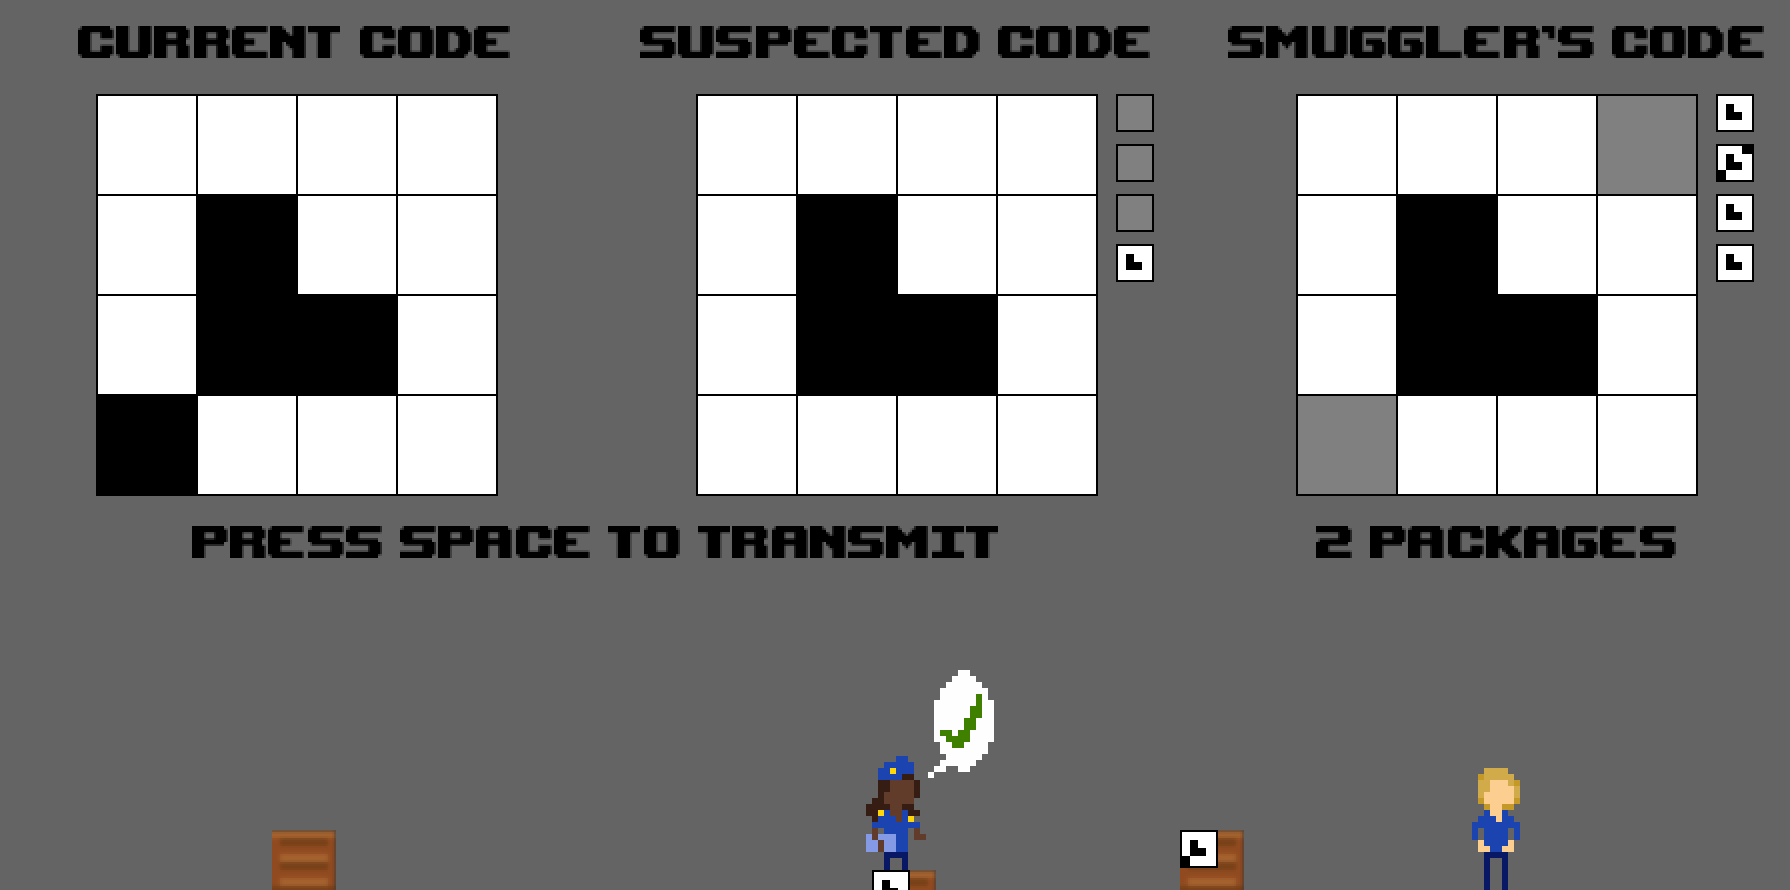
\includegraphics[width=0.45\textwidth]{images/contrabot}
\caption{{\sc Contrabot} interface: player input code on the left; inspector learned code in the middle; smuggler learned code on the right. 
Agent memories are shown as the set of smaller codes along the right of the larger central codes.}
\label{fig:contrabot}
\end{figure}

{\sc Contrabot}\footnote{\url{https://github.com/gamesbyangelina/contrabot}} (Figure \ref{fig:contrabot}) is a game based on agents that learn abstract codes with gameplay based on understanding, playing against and deceiving a machine learning system.
%
Players act as a smuggler trying to label boxes to communicate with a contact on the other side of a customs checkpoint.
The smuggler is trying to learn the code players use to indicate a box is contraband---but an inspector is randomly checking the same boxes.

The game mechanics revolve around how the smuggler and inspector agents learn to check codes based on codes they have seen.
These agents have two main processes: learning codes and matching new codes against their learned code.
Both agents generalize patterns from example codes---using a form of least general generalization---in their memory to then try to match new codes to these learned patterns.
The inspector has a larger memory than the smuggler and gameplay is based on using reverse-engineering how learning works to take advantage of the smuggler forgetting old patterns more quickly than the inspector.
%
The generalization process is simple, when comparing all codes seen the agents memorize exact matches for black or white tiles and generalizing to gray tiles if a position has been occupied by both colors.
Despite this simplicity the design accommodates many levels of difficulty and risk-reward considerations for players based on the size of the codes used and memory capacities of each agent.

We designed {\sc Contrabot} gameplay around risk-reward considerations for the player.
Both agents start with an empty learned code and empty memory. 
The smuggler learns from the first crate inspected and only retains a memory of the 4 most recent codes inspected. 
The inspector initially only has a random chance to inspect creates; after the inspector chooses to check a crate it begins learning and can either randomly check crates or check crates due to matching.
The inspector has an infinite memory, meaning the inspector will eventually learn a code that matches any new code (this ends the game).
After both agents have learned some code, gameplay revolves around creating codes that the inspector will not check (modulo random checks), but that the partner will check.
The number of crates the player passes to the smuggler serves as a score as the game will eventually end once the inspector learns to match all crates.
While simple, this design highlights how understanding the ways a machine learning algorithm works can be the core part of playing and succeeding at a game: in this case mastering the code learning algorithm to both avoid failure (inspector checks) and achieve success (smuggler checks).


\section{What Did You Do?}
\begin{figure}[tb]
\centering
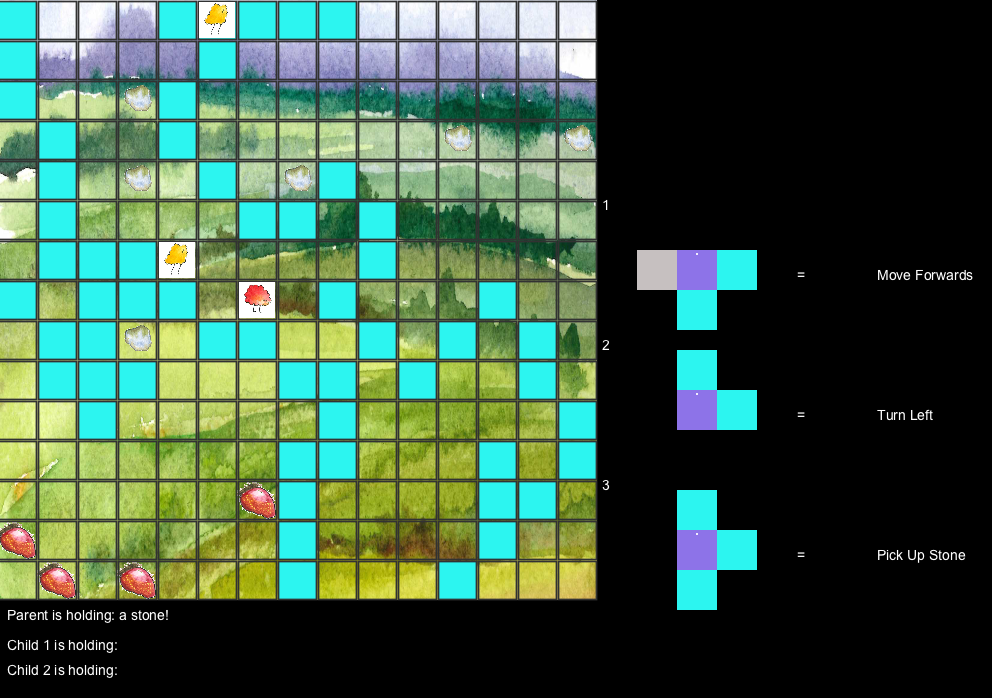
\includegraphics[width=0.45\textwidth]{images/WDYD}
\caption{{\sc What Did You Do?} interface: game world on the grid; rules learned by the child on right pane.}
\label{fig:WDYD}
\end{figure}

{\sc What Did You Do?}\footnote{\url{https://github.com/gamesbyangelina/whatareyoudoing}} (Figure \ref{fig:WDYD}) is a game based on indirectly training and directly editing a child AI agent to complete in-game tasks without the child dying along the way.
Players control a parent shrub attempting to raise an AI-controlled child agent in a simple environment.
The challenge derives from the child not being directly controlled by the player: the child learns behavioral rules to mimic the parent (player).
The game is turn-based and takes place in a grid world populated with helpful items (e.g., food) and obstacles (e.g., impassable rivers and stones).

Players aim to guide their navigate obstacles in the environment to reach a destination with their child still alive.
Obstacles include fording impassable rivers by picking up stones and dropping them into the river.
Parents may pick up objects or eat food to restore their energy level---depleting either the parent or child energy fully ends the game.
The environment is also more hazardous to the child than the parent: children may be crushed by dropping a stone on themselves after attempting to carry it too long or may drown in rivers.

The child observes the parent and learns rules of the form ``when surrounded with certain objects, perform a given action.''
For example, the child could learn a rule that when standing with a stone to the left and a pond behind, move forward.
Or if in front of a strawberry, pick it up.
Rules are re-learned every ten turns, and there is no limit to how many rules can be learned---this depends only on how many regularities the rule learning algorithm can find within the recent history of what the parent has
done.
The rule learning algorithm is a simple brute force search for all rules that can be constructed from recent activity; if using longer action histories or more actions, this could be replaced with the a priori rule learning algorithm.

We designed the rule learning system to play off food scarcity in the environment and the available hazards to the child.
On any turn the player may remove rules from the child's mind by spending energy from the parent.
Replacing energy requires food, meaning any adjustments made to keep the child from inadvertently harming itself comes at the cost of limited resources to stay alive.
Thus, promising courses of action can introduce trade-offs because your children are watching and could learn the wrong things.
For example, one might want to approach a stone from the opposite direction than what the shortest path would suggest, to avoid that the child sees regularities.
However, this takes more time and allows the child to potentially learn other bad behavior in the meantime.
These trade-offs induce players to explicitly reason about how the children learn and how to manage in-game resources around that learning.

\section{Discussion}
These games raise interesting problems with presenting machine learned knowledge to the player.
In {\sc Contrabot} learned codes are color-coded and the history of examples can be explicitly shown to the player for the smuggler (but only partially shown for the inspector).
Players can readily learn the visual language of the game, but not understand the gameplay implications of code choices.
At the same time the code language is very simple and can quickly become boring.
The way {\sc What Did You Do?} presents learned partial rules that may not be thought of as 'knowledge' to a human player unfamiliar with machine learning (such as what to do when a rock is to your left, but not what to do in the general case of being adjacent to rocks).
This means that editing knowledge can be exhausting, since there may be multiple cases that are all undesirable, which need to be manually removed when to the player they may seem to all stem from the same original case.
%
The presentation of machine learned knowledge both in {\sc Contrabot} and {\sc What Are You Doing?} presents interesting possibilities of how to use these technique in future game projects, and indicates the richness of new ideas to be found in applying these patterns to new aspects of gameplay.

%\cite{smith2012:endlessweb}

%\bibliographystyle{abbrv}
%\bibliography{../latex/lib}

\end{document}